\documentclass[tikz,border=10pt]{standalone}
\usepackage{tikz}
\usetikzlibrary {angles,quotes,arrows.meta, calc, intersections}
\usetikzlibrary{decorations.markings}
\tikzset{%
  ->-/.style={decoration={markings, mark=at position 0.7 with {\arrow{>[scale = 1, length=3]}}},
              postaction={decorate}},
}

\begin{document}
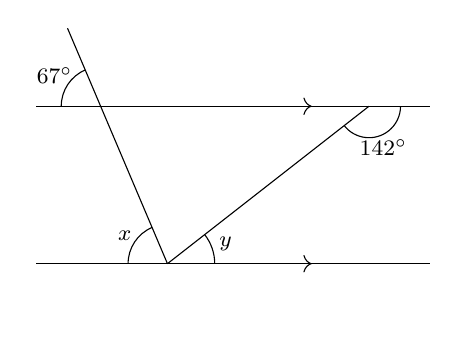
\begin{tikzpicture}[scale = 1]
    \coordinate (A) at (0,0);
    \coordinate (B) at (5,0);
    \coordinate (C) at (0,2);
    \coordinate (D) at ( 5,2);
    \coordinate (E) at (0.9,-0.6);
    \path (E) -- ++(38:4cm) coordinate (F);

    %parallel lines
    \draw[->-] (A) -- (B);
    \draw[->-] (C) -- (D);
    
    \coordinate (X) at (intersection cs:first line={(A)--(B)}, second line={(E)--(F)});
    \coordinate (Y) at (intersection cs:first line={(C)--(D)}, second line={(E)--(F)});
    
    
    %traversal line EF
    \draw (X) -- (Y);

    \draw[name path=leg1] (X) -- ($(X)!1!75:(Y)$) coordinate (N);
    \coordinate (Z) at (intersection cs:first line={(C)--(D)}, second line={(N)--(X)});
    
    % Draw the angle between lines
    \pic [draw, "\footnotesize $67^\circ$ ", angle eccentricity=1.4, angle radius=0.5cm] {angle = N--Z--C};
    \pic [draw, "\footnotesize $x$ ", angle eccentricity=1.3, angle radius=0.5cm] {angle = N--X--A};
    \pic [draw, "\footnotesize $142^\circ$ ", angle eccentricity=1.4, angle radius=0.4cm] {angle = X--Y--D};
    \pic [draw, "\footnotesize $y$ ", angle eccentricity=1.3, angle radius=0.6cm] {angle = B--X--Y};
    
\end{tikzpicture}

\end{document}
